\documentclass[a4paper,openright,12pt]{article}
\date{}
\usepackage[spanish]{babel}
\usepackage{graphicx}
\usepackage{amssymb}
\usepackage{fancyhdr}
\usepackage{multirow}
\usepackage[utf8]{inputenc}
\usepackage{fancyhdr}

\begin{document}
\renewcommand{\tablename}{Tabla}
\renewcommand{\listtablename}{\'Indice de tablas}
\renewcommand{\headrulewidth}{0.3pt}
\renewcommand{\footrulewidth}{0.3pt}
\newpage

\begin{titlepage}
	\begin{center}
		\vspace*{-1in}
		\begin{figure}[htb]
			\begin{center}
				
\includegraphics[width=10cm]{ug}
			\end{center}
		\end{figure}
		\vspace*{0.1in}
		\begin{Large}
			Ingenier\'ia en Sistemas, Inform\'atica y \\Ciencias de la Computaci\'on\\
		\end{Large}
		\vspace*{0.2in}
		\begin{Large}
			Seminario Profesional II\\
		\end{Large}
		\vspace*{0.9in}
		\begin{LARGE}
			\textbf{\LARGE MAYALENG} \\
			\begin{figure}[htb]
				\begin{center}
					
\includegraphics[width=4cm]{ml}
				\end{center}
			\end{figure}
		\end{LARGE}
		\vspace*{0.9in}
		\begin{large}
			Autores:\\
			Douglas Figueroa \\
			Alexander Baquiax
		\end{large}
		\vspace*{0.3in}
		\\
		\rule{90mm}{0.1mm}\\
		\begin{large}
			Supervisado por: \\
			Ing. Jack Trachtenberg \\
			Ing. Axel Benavides
		\end{large}
	\end{center}
\end{titlepage}
\newpage

\tableofcontents

\cleardoublepage
\listoffigures

\cleardoublepage
\listoftables

\newpage

\pagestyle{fancy}
\rfoot{
\includegraphics[width=.08\textwidth]{ml}}
\lfoot{MayaLeng}
\section{Introducci\'on}
Mayaleng m\'as que una aplicaci\'on es un algoritmo con la capacidad de recibir un input, en nuestro caso, una palabra, una frase, un p\'arrafo, una cantidad de texto muy grande, en espa\~nol y retornar un output, (el texto de entrada), en una lengua maya. \\

Una herramienta de traducci\'on y para conocimiento de la cultura de Guatemala.
\newpage

\section{Objetivos}
\subsection{Objetivo General}
Crear una herramienta de traducci\'on de lenguas mayas.
\subsection{Objetivos Espec\'ificos}
\begin{itemize}
    \item Crear una aplicaci\'on m\'ovil (Android y iOS) para traducir lenguas mayas.
    \item Dar a conocer la cultura de nuestro pa\'is Guatemala.
    \item Brindar la capacidad a profesores y personas en general de traducir documentos para facilitar su trabajo en los lugares d\'onde imparten clases dentro de nuestro pa\'is y los cuales no dominan el espa\~nol.
\end{itemize}
\newpage

\section{El Problema}
\subsection{¿Cuál es el problema?}
El problema analizado para querer desarrollar esta herramienta fue desde un punto de vista cultural, ya que en Guatemala existen muchas lenguas mayas, de las cuales pocas personas en el pa\'is dominan como m\'inimo una. Estas forman parte de nuestro patrimonio cultural. Alrededor del mundo Guatemala es conocida por los puntos tur\'isticos con los que contamos, regularmente estos se encuentran en los departamentos donde al menos existe una lengua Maya.  Como guatemaltecos deber\'iamos de poder comunicarnos con la gente de nuestro pa\'is, ya que en algunos departamentos no se habla mucho en espa\~nol sino que hablan en una lengua maya, sin embargo ese no es el caso. No hemos encontrado tantas herramientas claras que nos faciliten dicha tarea, queremos ser de los primeros en brindar dicha herramienta.\\

En este momento sugerimos kaqchikel, la forma en que solucionamos el problema de la comunicación es teniendo una aplicación m\'ovil la cu\'al har\'a una traducción en nuestro idioma natal a kaqchikel, sencillamente quien utilice la aplicación deberá ingresar el texto y en una casilla aparte aparecer\'a la traducci\'on del texto, algo similar a google translate.\\

Le ahorraremos al usuario tener que escribir algunas de las frases o palabras m\'as utilizadas, ya que tendremos una secci\'on donde diremos como se dicen esas frases, cosas b\'asicas como saludar, despedirse, hasta algo m\'as formal, un ejemplo ser\'ia preguntar d\'onde se encuentra el bano, preguntar el nombre de una persona y frases similares.\\
\newpage

\section{Estudio de Factibilidad}
\subsection{Factibilidad Funcional}
\subsubsection{Encuesta}
\begin{enumerate}
	\item ¿Le gustaría aprender una lengua maya?\\
	SI \rule{10mm}{0.1mm}  \hspace{5cm} NO \rule{10mm}{0.1mm}
	\item ¿Al visitar un departamento en Guatemala le gustaría poder comunicarse con personas que solamente conocen una lengua maya?	\\
	SI \rule{10mm}{0.1mm}  \hspace{5cm} NO \rule{10mm}{0.1mm}
	\item ¿Cree que aprender sobre la cultura de nuestro país es importante?\\
	SI \rule{10mm}{0.1mm}  \hspace{5cm} NO \rule{10mm}{0.1mm}
	\item ¿Usaría una aplicación móvil para aprender cosas básicas sobre lenguas mayas?\\
	SI \rule{10mm}{0.1mm}  \hspace{5cm} NO \rule{10mm}{0.1mm}
	\item ¿Pagaría por la aplicación?\\
	SI \rule{10mm}{0.1mm}  \hspace{5cm} NO \rule{10mm}{0.1mm}
	\item ¿Estaría dispuesto a invertir 10 minutos al día para conocer una lengua maya?\\
	SI \rule{10mm}{0.1mm}  \hspace{5cm} NO \rule{10mm}{0.1mm}
	
\end{enumerate}
\subsubsection{Resultados de Encuesta}
Hola\\
Hola\\
Hola\\

\begin{table}[h]
	\resizebox*{14cm}{!}{
	\begin{tabular}{|r|c|c|c|c|}
	\hline
	Funcionalidad & Google Translate & Glosbe.com & Profesor & MayaLeng\\
	\hline
	Traducci\'on de palabras & \checkmark & \checkmark & \checkmark & \checkmark\\
	\hline
	Traducci\'on	 bidireccional & \checkmark & x & \checkmark & x\\
	\hline
	Traducci\'on de frases  & \checkmark & x & \checkmark & \checkmark\\
	\hline
	Traducci\'on precisa & \checkmark & x & \checkmark & \checkmark\\
	\hline
	Herramienta de traducci\'on de documentos & \checkmark & x & \checkmark & \checkmark\\
	\hline
	\end{tabular}}
\caption{Comparativa de Funcionalidades}
\end{table}

\begin{table}[h]
	\resizebox*{14cm}{!}{
	\begin{tabular}{|r|c|c|c|c|}
	\hline
	Caracter\'istica & Google Translate & Glosbe.com & Profesor & MayaLeng\\
	\hline
	Descripci\'on de palabras & x & \checkmark & \checkmark & x\\
	\hline
	Intuitivo & \checkmark & x & \checkmark & \checkmark\\
	\hline
	Es gratis  & \checkmark & \checkmark & x & \checkmark\\
	\hline
	Siempre disponible & \checkmark & \checkmark & x & \checkmark\\
	\hline
	F\'acil de obtener/contactar & \checkmark & \checkmark & x & \checkmark\\
	\hline
	\end{tabular}}
\caption{Comparativa de Caracter\'isticas}
\end{table}

\subsection{Factibilidad T\'ecnica}
Pretendemos aprovechar el apogeo de los m\'oviles y tratar de crear una buena oportunidad para introducir nuestro proyecto.\\
Actualmente existen dos grandes sistemas operativos que domina la industria de los m\'oviles:. iOS y Android. Estamos conscientes de que desarrollar de forma nativa para ambas plataformas nos representar\'ia un poco m\'as de tiempo, que implicar\'ia restarle tiempo a la parte que en verdad es importante. Por lo cual usaremos IONIC, framework que nos permite desarrollar de manera sencilla aplicaciones m\'oviles usando las tendencias de Responsive Web Design. \\

Lo interesante de este proyecto no radica en la aplicaci\'on m\'ovil, de hecho la aplicaci\'on s\'olo ser\'a una forma de consumir nuestro verdadero sistema.\\

La idea de este proyecto radica en hacer un compilador que pueda usar una gram\'atica y una fuente de palabras de esa gram\'atica, y traducir de ellas las palabras al español. En pocas palabras nuestro proyecto radica en hacer un compilador de idiomas mayas.\\

Durante el transcurso de nuestra carrera ya hicimos un compilador, con todas las fases b\'asicas que uno de ellos debe tener. Ahora nos pusimos el reto de hacer un compilador gen\'erico. Para esta primera versi\'on usaremos dos idiomas Mayas.\\

Creemos tener los conocimientos necesarios para la construcci\'on de esto. Uno de los inconvenientes m\'as grandes era que ninguno de los dos sabemos hablar un idioma Maya, pero nos apoyamos en la documentaci\'on que distintas personas a lo largo de la historia han construido.\\ 

La idea es construir un API al que se le pueda dar como input un texto, p\'arrafo, documento y que la salida sea otro documento pero con texto traducido. Ahora tenemos una base de datos con 15 mil palabras aproximadamente del Kaqchikel. La DB esta montada en un DBMS MySQL. El API fue construido en Symfony2.\\

El core de traducci\'on ser\'a hecho en Java,  usando herramientas de parseo y an\'alisis sint\'actico como Flex.

\subsubsection{Conclusión}
La tecnología utilizada cubre con las necesidades para el proyecto, nos ayuda a que las tareas sean optimizadas, utilizando menos recursos y optimización de tiempo, lo cuál es un punto muy importante a considerar.

\subsection{Factibilidad Econ\'omica}
Bas\'andonos en nuestra calendarizaci\'on de tareas para el desarrollo del proyecto, hemos estimado los siguientes costos para el desarrollo de la aplicaci\'on, los gastos son a nivel de costo de servidor, por compra del dominio, licencias para subir aplicaci\'on y gastos en papel, en impresi\'on del manual de usuario.\\

\begin{table}[h]
	\resizebox*{15cm}{!}{
	\begin{tabular}{|l|c|r|}
	\hline
	Tarea & D\'ias Trabajados & Costo (Q.)\\
	\hline
	Configurar servicios iniciales.\\
	Montar la base de datos del proyecto anterior.
	& 7 
	& 70\\
	\hline
	Generar la documentación adecuada del algoritmo de traducción.\\
	Extraer las reglas de la gramática de libros y textos.
	& 7 
	& 130\\
	\hline
	Lanzar primera versión del API.\\
	Traducción de oraciones sencillas.\\
	App consumiendo API.
	& 7
	& 192\\
	\hline
	Documentación final y manual de usuario.\\
	Lanzamiento final.
	& 7
	& 50\\
	\hline
	Total 
	&
	& 442\\
	\hline
	\end{tabular}}
\caption{Factibilidad Econ\'omica}
\end{table}

\subsubsection{Conclusión}
El costo monetario del desarrollo de nuestra herramienta no es tan alto debido a qué contamos con las herramientas para prueba (teléfono con Android y iPad) y pocas cosas son en las que hemos invertido.
\newpage

\section{Anexo}
\subsection{Calendarización}
\begin{figure}[h]
  \centering
    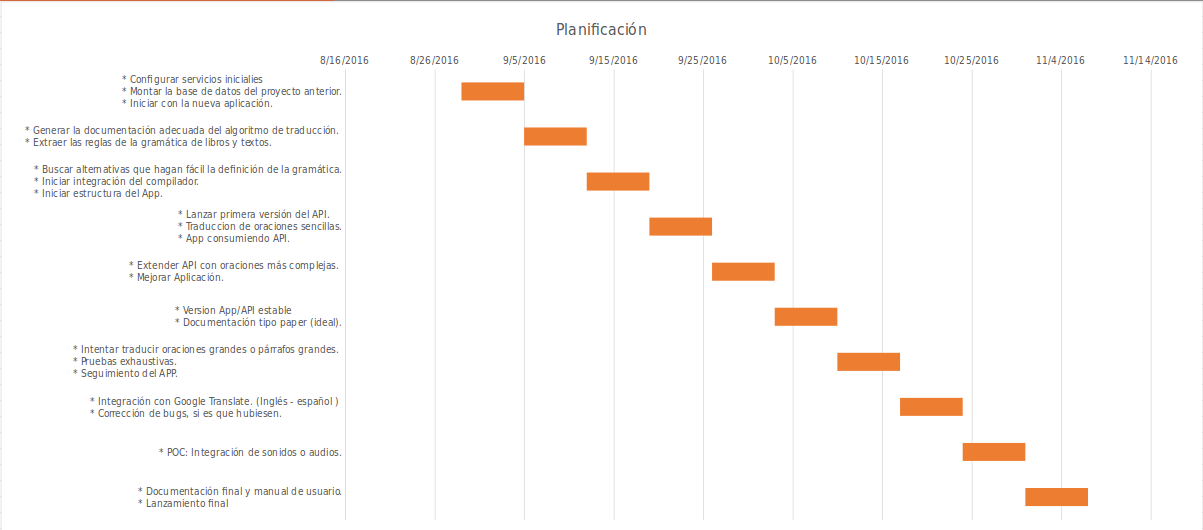
\includegraphics[width=1.0\textwidth]{Gantt}
  \caption{Diagrama de Gantt}
  \label{fig:gantt}
\end{figure}

\newpage
\subsection{Diagrama Entidad-Relación}
\begin{figure}[h]
	\centering
	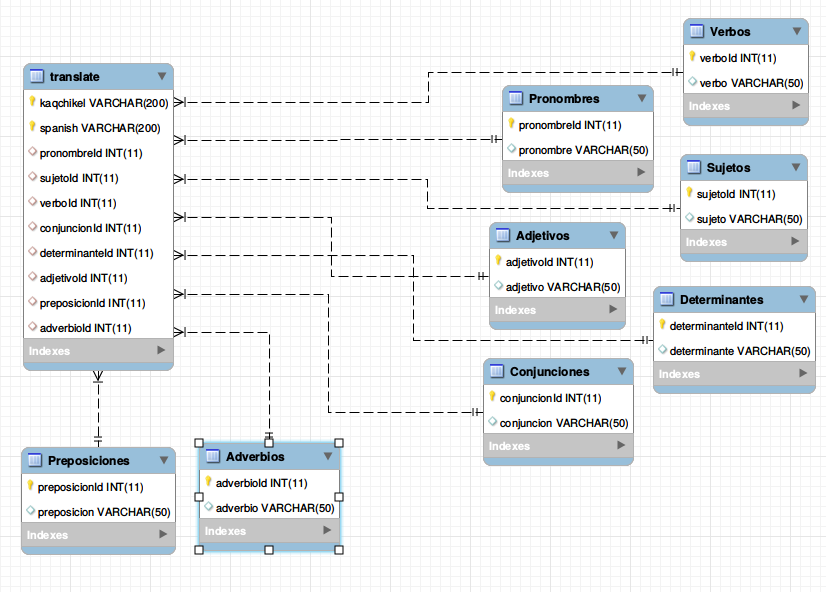
\includegraphics[width=0.9\textwidth]{er}
	\caption{Diagrama Entidad Relación}
	\label{fig:er}
\end{figure}
La base de datos está compuesta por una tabla principal que contiene el vocabulario, con la palabra en español y su traducción a kaqchikel, tenemos llaves foráneas a cada palabra asociada a su estructura gramatical (sujeto, verbo, adjetivo, etc), en el diagrama se ve que la información estará duplicada, estará en la tabla del vocabulario y en las estructuras gramaticales, sin embargo, ya que el usuario no realizará ningún insert a la base de datos, ésta no crecerá descontroladamente ya que solo nosotros controlaremos la información que allí se encuentre, este diseño nos ayudará a que nuestra aplicación sea más rápida, tendremos un costo en espacio pera ganaremos velocidad.
\newpage

\section{Glosario}
\noindent \textbf{Kaqchikel: } lengua maya, parte de la familia lingüística mayense. \\\\
\textbf{iOS: } sistema operativo móvil de Apple \\\\
\textbf{Android: } sistema operativo móvil de Google \\\\
\textbf{Framework: } conjunto estandarizado de conceptos, prácticas y criterios para enfrentar y resolver nuevos problemas de índole similar. \\\\
\textbf{Responsive Web Design:  adaptar la apariencia de las páginas web al dispositivo que se esté utilizando para visualizarlas. }  \\\\
\textbf{API:  } utilizada por otro software como una capa de abstracción \\\\
\textbf{DB: } base de datos \\\\
\textbf{DBMS: } programa que permite almacenar y posteriormente acceder a los datos de forma rápida y estructurada.\\\\
\textbf{MySQL: }  sistema de gestión de bases de datos relacional \\\\
\textbf{Symfony2: } framework diseñado para optimizar el desarrollo de aplicaciones web\\ \\
\newpage

\pagestyle{fancy}
\end{document}